\documentclass{article}
\usepackage[utf8]{inputenc}
\usepackage[document]{ragged2e}
\usepackage{algpseudocode}
\usepackage[]{algorithmicx}
\usepackage{amsmath}
\usepackage{amsthm}
\usepackage{amssymb}
\usepackage[]{listings}
\usepackage{graphicx}
\usepackage{hyperref}
\usepackage{flafter}
\usepackage{subfig}
\usepackage{dsfont}
\usepackage[T1]{fontenc}


\begin{document}

\begin{titlepage}
	\centering
	
\includegraphics[width=0.15\textwidth]{IIIT-B_logo.jpg}\par\vspace{1cm}
	{\scshape\LARGE International Institute of Information Technology, Bangalore \par}
	\vspace{1cm}
	{\scshape\Large Milestone 4 - Clustering and Association rules\par}
	{\Large  DS 707 Data Analytics\par}
	\vspace{1.5cm}
	{\huge\bfseries Cryptocurrency Analysis and Blockchain Understanding \par}
	\vspace{2cm}
	{\Large\itshape Akanksha Dwivedi - MT2016006\par}
	{\Large\itshape Hitesha Mukherjee - MS2016007\par}
	{\Large\itshape Nayna Jain - MS2017003\par}
	{\Large\itshape Tarini Chandrashekhar - MT2016144\par}
	\vfill
	Instructors : \par
	Prof. Ramanathan Chandrashekhar
	\par
	Prof. Uttam Kumar

	\vfill
% Bottom of the page
	{\large \today\par}
\end{titlepage}
\tableofcontents
\justify
\newpage

\section{Background}
As with stock market, cryptocurrency is a growing investment area for the daily traders and investors. Cryptocurrency is very new and still stabilizing because of which it is very volatile in nature and might get affected by different factors. In such an environment, it is very difficult to predict the price movement of cryptocurrencies. Since the trend and investment point of view is similar to stock market, the established techniques used in stock market prediction, are considered
for cryptocurrency.

\section{Trial \& Error on Classification Model}
To improve the accuracy of the classification models built, the following criteria were used:
\subsection{Application of Dimensionality Reduction}
According to the Wikipedia, dimensionality reduction or dimension reduction is the process of reducing the number of random variables under consideration by obtaining a set of principal variables. The main linear technique for dimensionality reduction, principal component analysis, performs a linear mapping of the data to a lower-dimensional space in such a way that the variance of the data in the low-dimensional representation is maximized. In practice, the covariance (and sometimes the correlation) matrix of the data is constructed and the eigen vectors on this matrix are computed. The eigen vectors that correspond to the largest eigenvalues (the principal components) can now be used to reconstruct a large fraction of the variance of the original data. Moreover, the first few eigen vectors can often be interpreted in terms of the large-scale physical behavior of the system[citation needed][why?]. The original space (with dimension of the number of points) has been reduced (with data loss, but hopefully retaining the most important variance) to the space spanned by a few eigenvectors.
We used 'prcomp' function to compute the principal components which uses Singular Value Decomposition technique. The number of principal components were selected from the scree plot and elbow curve on the respective datasets, which clearly highlights the important principal components. After choosing the principal components, the data was again projected back(with reduced dimension) to be used for classification models. We could achieve only a maximum of 58\% accuracy after applying PCA.
\newpage

\begin{figure}[ht]
	\centering
	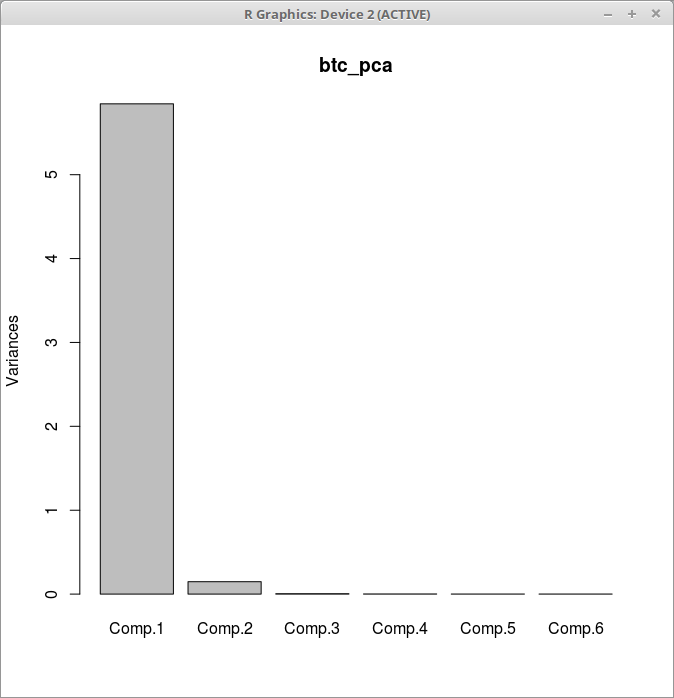
\includegraphics[width = 6 cm]{bitcoin_pca.png}
	\caption{Scree plot of principal components of bitcoin}
	\label{fig: btc_pca}
\end{figure}

\begin{figure}[ht]
	\centering
	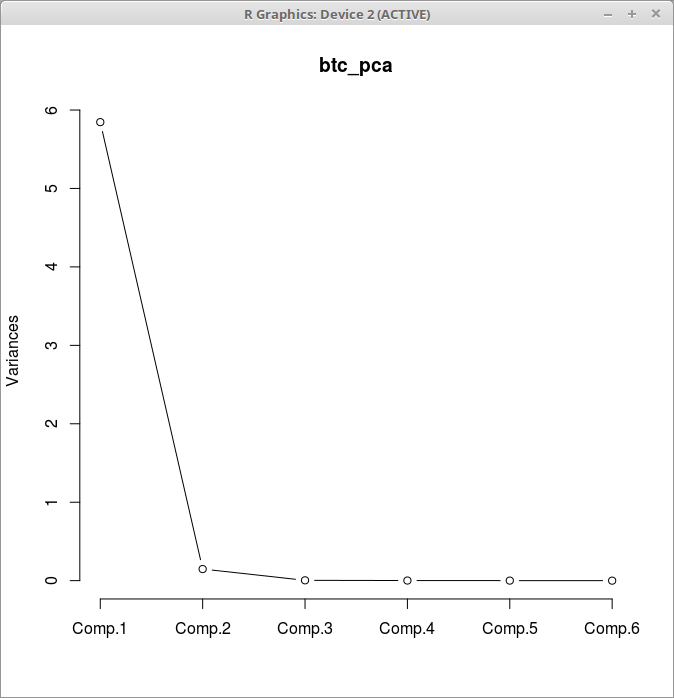
\includegraphics[width = 6 cm]{bitcoin_pca_elbow.png}
	\caption{Elbow Curve on bitcoin dataset}
	\label{fig: btc_pca_elbow}
\end{figure}
\newpage

\begin{figure}[ht]
	\centering
	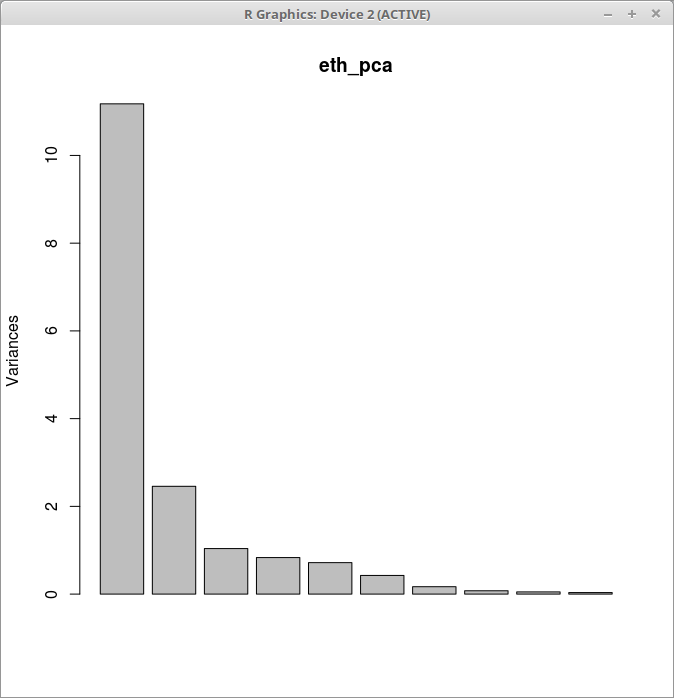
\includegraphics[width = 6 cm]{ethereum_pca.png}
	\caption{Scree plot of principal components of ethereum}
	\label{fig: eth_pca}
\end{figure}

\begin{figure}[ht]
	\centering
	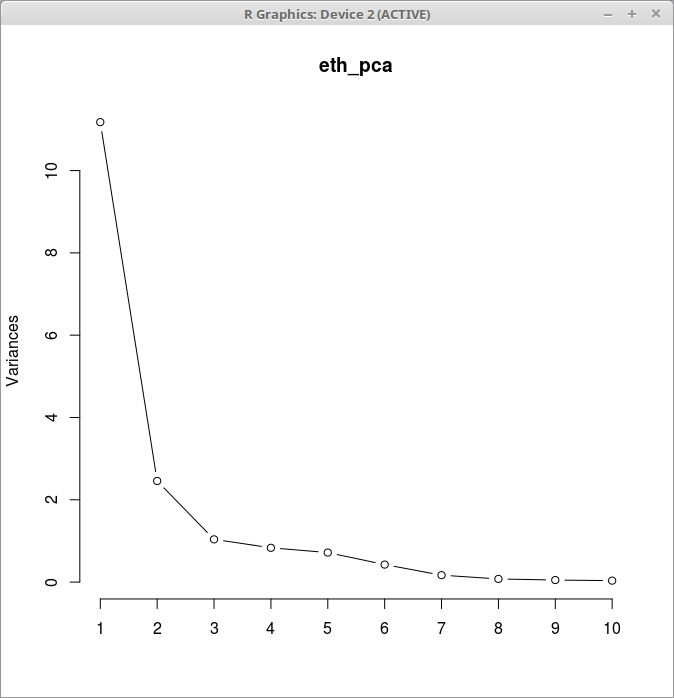
\includegraphics[width = 6 cm]{ethereum_pca_elbow.png}
	\caption{Elbow Curve on ethereum dataset}
	\label{fig: eth_pca_elbow}
\end{figure}

\newpage
\subsection{K-Fold Loss Cross Validation Strategy}
Cross-validation is a technique to evaluate predictive/classiification models by partitioning the original sample into a training set to train the model, and a test set to evaluate it. In k-fold cross-validation, the original sample is randomly partitioned into k equal size subsamples. Of the k subsamples, a single subsample is retained as the validation data for testing the model, and the remaining k-1 subsamples are used as training data. The cross-validation process is then repeated k times (the folds), with each of the k subsamples used exactly once as the validation data. The k results from the folds can then be averaged (or otherwise combined) to produce a single estimation. The advantage of this method is that all observations are used for both training and validation, and each observation is used for validation exactly once. For classification problems, one typically uses stratified k-fold cross-validation, in which the folds are selected so that each fold contains roughly the same proportions of class labels.
In our case, we have use Leave-One-Out cross validation strategy, in which only one datapoint is left as testing point which the remaining are used for training. This process is repeated for 10 times i.e. in k folds. The plot below shows the different combinations of hyper-parameters used and the respective accuracy achieved with model.
\begin{figure}[ht]
	\centering
	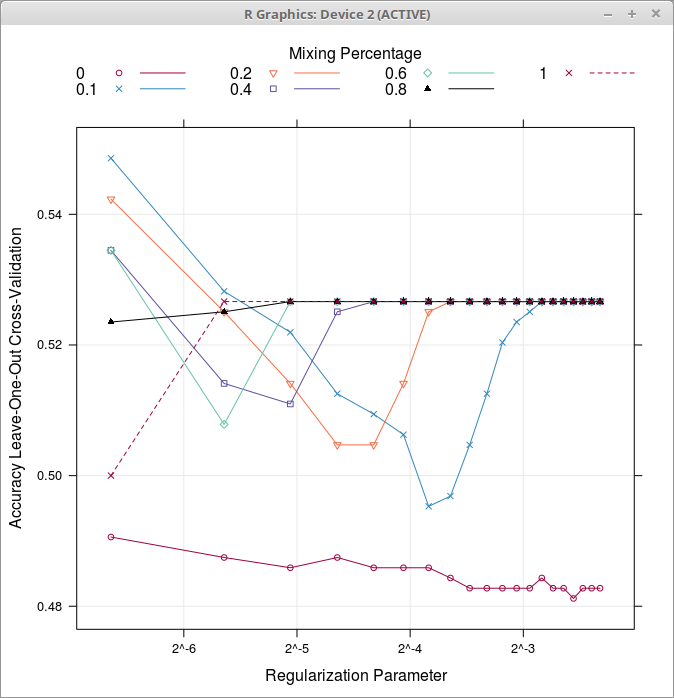
\includegraphics[width = 6 cm]{loocv.png}
	\caption{Plot of Leave One Out Cross Validation Accuracy with regularization parameters}
	\label{fig: loocv}
\end{figure}
A maximum accuracy of 54\% was achieved with this strategy.
From the above trial and error strategies, we inferred that this low accuracy of the classfication models might be due to insufficient number of datapoints and the granularity of datapoints available.

\section{Clustering Techniques}
\subsection{K-Means Clustering}
[1][2] refers to the papers which shows how clustering is used in the process of stock price prediction. We have applied similar techniques from [1] for the cryptocurrency forecasting. [1] discusses three steps for forecasting:
\begin{itemize}
	\item Normalizing the data.
	\item K-means clustering of the normalized data to identify the outliers.
	\item ARIMA model for forecasting on clustered data.
\end{itemize}
This is done to see how clustering is applied to remove the outliers from the clusters.
It is a centroid based partitioning technique that uses the centroid of a cluster, C$_{i}$ to represent the cluster. Conceptually, the centroid of a cluster is its center point. This algorithm requires to specify the number of clusters (k) beforehand. This method is not guaranteed to converge to the global optimum and often terminates to a local optimum.
The algorithm on Close/High attributes of the daily prices. Out of cluster values from 3, 4 and 5, we found that cluster values of 4 and 5 give similar values. Hence, we attempt to identify the outliers based on these attributes, with 4 clusters.

\begin{figure}[ht]
	\centering
	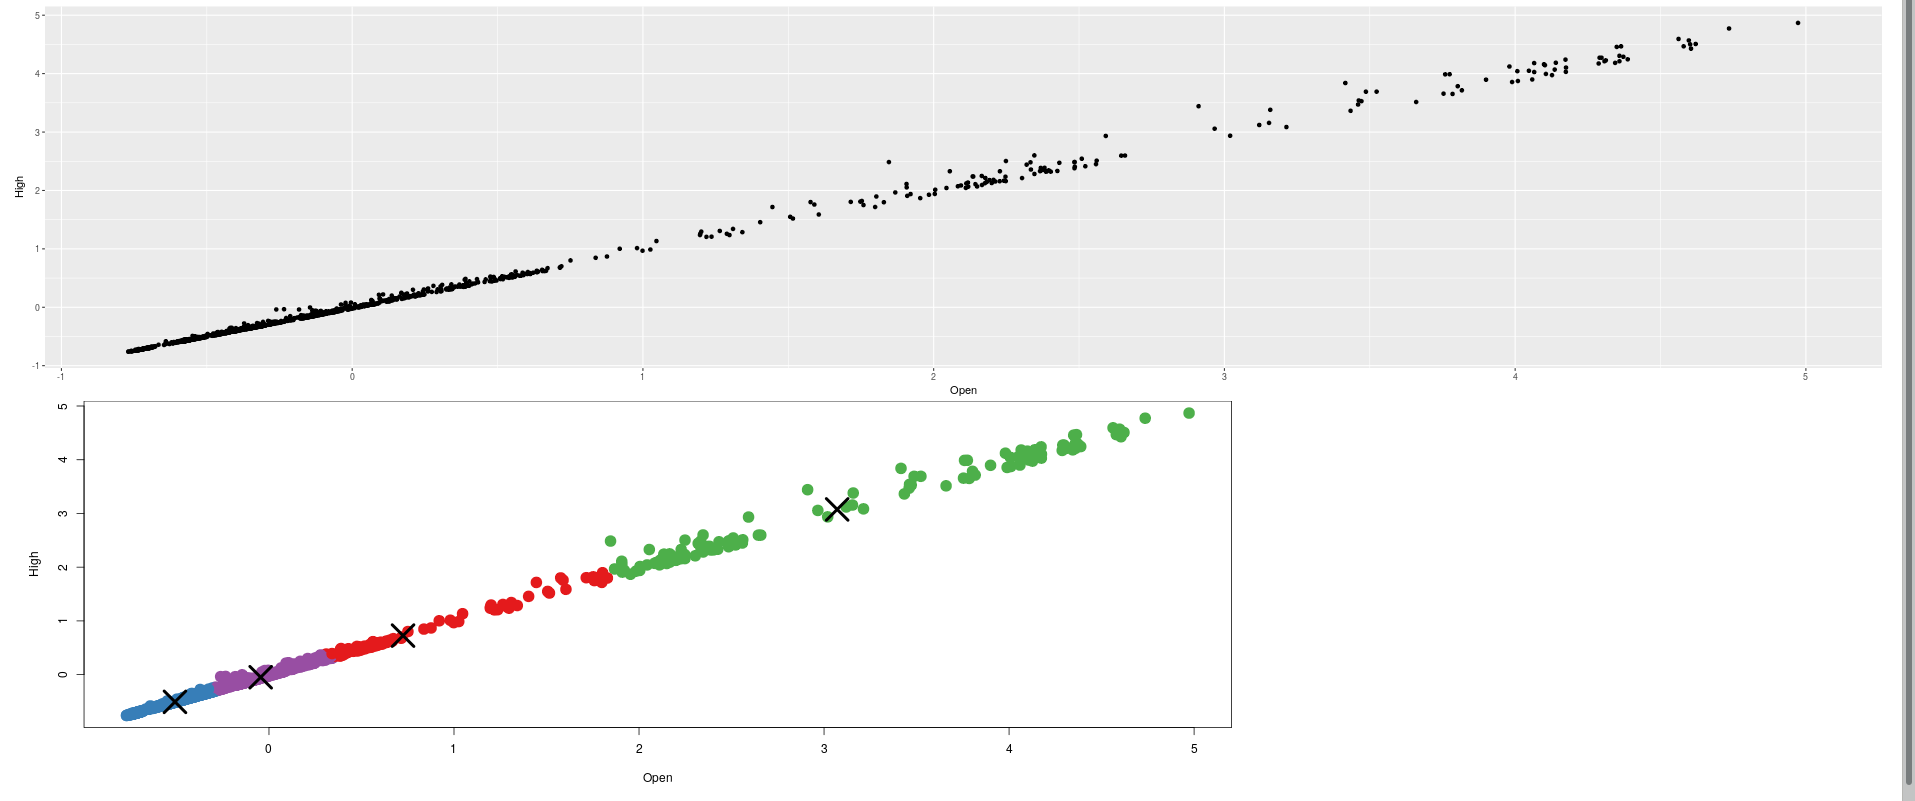
\includegraphics[width= 10cm]{KMeansClustering.png}
	\caption{Before and After K Means Clustering}
	\label{fig:kmeansclustering}
\end{figure}

\subsection{Hierarchical Clustering}
Hierarchical clustering algorithm called CHAMELEON that measures the similarity of two clusters based on a dynamic model. In the clustering process, two clusters are merged only if the inter-connectivity and closeness (proximity) between two clusters are comparable to the internal inter-connectivity of the clusters and closeness of items within the clusters. We have considered the Bitcoin Data Set which has 24 features or attributes in it. We have extracted 16 important features and build a subset of the data. This dataset has been clustered using Chameleon. From the below figure we see that we have six clusters of different size, shape, and orientation, as well as random noise points and special artifacts such as streaks running across clusters.In this case CHAMELEON finds eleven clusters, out of which six of them correspond to the genuine clusters in the data set, and the rest contain outliers.\newline

\begin{figure}[h]
    \centering
    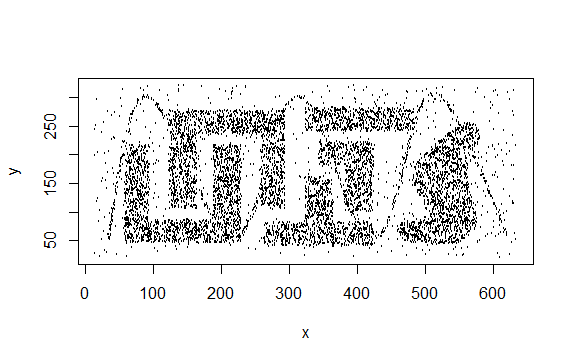
\includegraphics[width=10cm]{chameleonBitcoinFig1.png}
    \caption{Chameleon Clustering Bitcoin}
    \label{fig:my_label}
\end{figure}

The next data set is ethereum Dataset with 12 attributes. From Figure 8 we see it has eight clusters of different shape, size, and orientation, some of which are inside the space enclosed by other clusters. Moreover, it also contains random noise and special artifacts, such as a collection of points forming vertical streaks. In this case CHAMELEON also finds eleven clusters, out of which nine of them correspond to the genuine clusters, and the rest contain outlier points.

\begin{figure}[h]
    \centering
    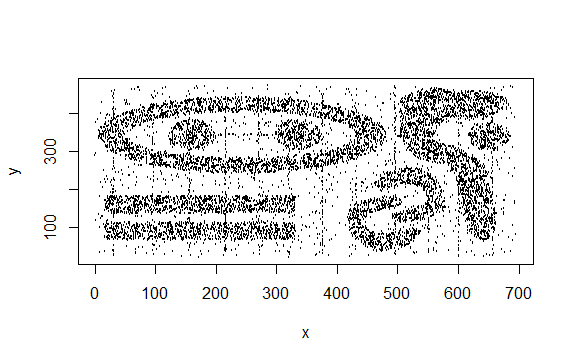
\includegraphics[width=10cm]{ChameleonEtheriumFig2.png}
    \caption{Chameleon Clustering Etherium}
    \label{fig:my_label}
\end{figure}

\newpage 
\subsection{Partition along medioids clustering(PAM) : CLARANS}
CLARANS (Clustering Large Applications based uponRANdomized Search ) was proposed to improve the quality and the scalability of CLARA. It combines sampling techniques with PAM.It does not confine itself to any sample at a given time. It draws a sample with some randomness in each step of the search.
\newline
\textbf{Advantages}
\begin {itemize}
\item Experiments show that CLARANS is more effective than both PAM
and CLARA.
\item Handles outliers 
\newline
\textbf{Disadvantages}
\item The computational complexity of CLARANS is O($n^2$), where n is the
number of objects.
\item The clustering quality depends on the sampling method
\end{itemize}

We take the Bitcoin Dataset into consideration. It has 16 attributes. We have considered 2 attributes(Market Price Label and Market Cap)  for CLARANS Clutering. From Figure 9, we observe that the Market Cap and Market Price varies almost in the same way for negative and positive values. It means that they are highly correlated. There is a similarity in their pattern, hence the clusters are based on similarity measure. We have used Euclidean Distance Parameter for Computation. 

\begin{figure}[h]
    \centering
    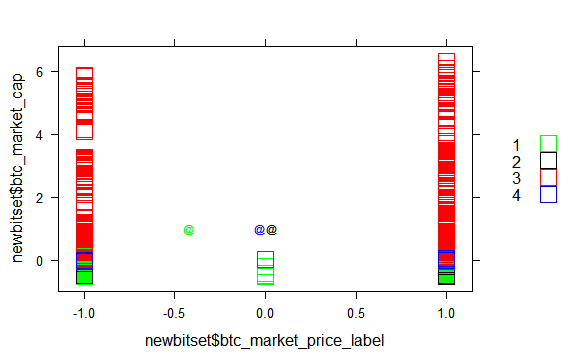
\includegraphics[width=10cm]{CLaransClusteringFig3.png}
    \caption{Clarans Clustering for Market Price and Market Cap }
    \label{fig:my_label}
\end{figure}

The next dataset we considered is the BitCoin Price Dataset which has 7 attributes. From below figure 10, we have considered 2 attributes(Volume and Market Cap) for CLARANS Clutering. We observe a certain randomness about the clusters. No similarity pattern is observed. The volume and Market Cap vary randomly.

\begin{figure}[h]
    \centering
    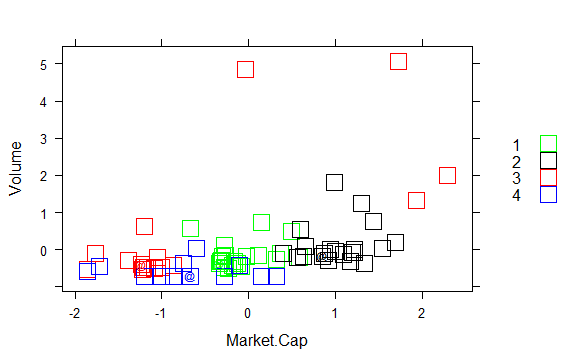
\includegraphics[width=10cm]{CLARANSMARCAPVOLFig4.png}
    \caption{Clarans Clustering for Market Cap and Volume }
    \label{fig:my_label}
\end{figure}

\newpage
\section{Density-Based Clustering : DBSCAN}
Density-based clustering is a technique that allows to partition data into groups with similar characteristics (clusters) but does not require specifying the number of those groups in advance. In density-based clustering, clusters are defined as dense regions of data points separated by low-density regions. Density is measured by the number of data points within some radius.\newline

\textbf{Advantages of density-based clustering:}
\newline
As mentioned above, it does not require a predefined number of clusters,clusters can be of any shape, including non-spherical ones,the technique is able to identify noise data (outliers).\newline

\newline

\textbf{Disadvantages:}
\newline
Density-based clustering fails if there are no density drops between clusters, it is also sensitive to parameters that define density (radius and the minimum number of points); proper parameter setting may require domain knowledge.

This algorithm works on a parametric approach. The two parameters involved in this algorithm are:
e - (eps) is the radius of our neighborhoods around a data point p.Using these two parameters, DBSCAN categories the data points into three categories:


\begin{itemize}
\item  minPts (K)- It is the minimum number of data points we want in a neighborhood to define a cluster.
\item Core Points: A data point p is a core point if Nbhd(p,eps) [eps-neighborhood of p] contains at least minPts; \mathopen|Nbhd(p,eps)|$\geq$ minPts.
Border Points: A data point *q is a border point if Nbhd(q, eps) contains less than minPts data points, but q is reachable from some core point p.
\item Outlier: A data point o is an outlier if it is neither a core point nor a border point. Essentially, this is the "other" class. \newline
\end{itemize}
The idea is to calculate, the average of the distances of every point to its k nearest neighbors. The value of k will be specified by the user and corresponds to MinPts.We have used K-Nearest Neighbour Algorithm to determine the K value (minPts) to be used as a parameter for the DBSCAN Algorithm. The minimum value obtained for K was 5. \newline

The value of epsilon is calculated in the following manner. The function kNNdistplot() [in dbscan package] can be used to draw the k-distance plot. k-distances are plotted in an ascending order. The aim is to determine the “knee”, which corresponds to the optimal eps parameter. \newline

A knee corresponds to a threshold where a sharp change occurs along the k-distance curve. From the below figure, It can be seen that the optimal eps value is around a distance of 0.15.
\newpage

\begin{figure}[h]
    \centering
    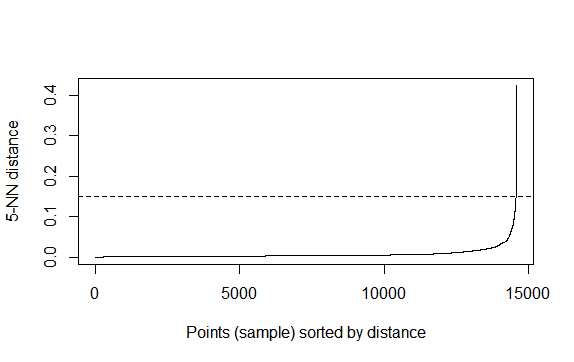
\includegraphics[width=10cm]{epswith2attrFig5.png}
    \caption{K-Distance Curve for determining Eps Value }
    \label{fig:my_label}
\end{figure}

We take the Bitcoin Dataset into consideration. It has 16 attributes. We have considered 2 attributes(Total Bitcoins and Market Cap) for DBSCAN Clustering.\newline

From the figure 12, the variation of Total Bitcoins and Market Cap is constant for negative values, but as the value increases, we observe a sharp spike after zero for total BitCoins with respect to the Market Cap. The blue Cluster has maximum density, it is densely connected and has maximum density reachable value. We observe there are two outliers in the dataset. \newline


\begin{figure}[h]
    \centering
    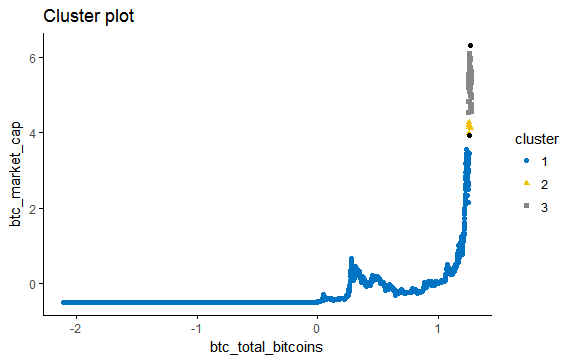
\includegraphics[width=10cm]{PlotMarCapTotCoinsFig6.png}
    \caption{DBSCAN Clustering for Total Coins and Market Cap }
    \label{fig:my_label}
\end{figure}

We have considered 2 attributes Total Bitcoins and Trade Volume for DBSCAN Clustering. From figure 13, we observe that there is sharp change in the value of Total Bitcoins and Trade Volume. Also there is an overlap of clusters(Blue Cluster and Gray Cluster).The entire Blue Cluster and some parts of the Gray Cluster can be considered as core points and the remaining parts of gray cluster are the Border Points. There are 2 points away from the clusters one is yellow point and the other single gray point, which can be termed as outliers. \newline

\begin{figure}[h]
    \centering
    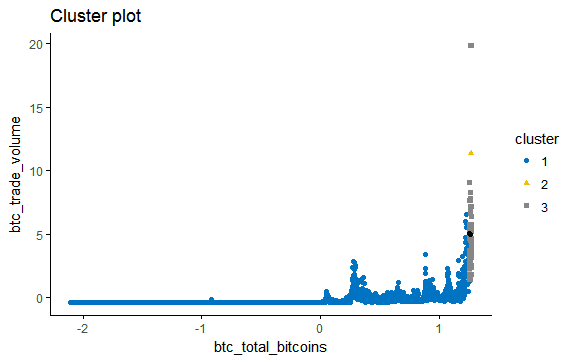
\includegraphics[width=6cm]{totbitcoinstradevolFig7.png}
    \caption{DBSCAN Clustering for Total Coins and Trade Volume }
    \label{fig:my_label}
\end{figure}

We have considered 2 attributes Market Cap and Trade Volume for DBSCAN Clustering. From Figure 14, we observe that the first cluster is very dense. The second and third clusters are very sparse. We observe that as the Market Cap increases the clusters become less denser, After the market cap and trade volume crosses the value of 5 in the x and y axis we observe very few points lie on that region. We can therefore conclude that both Market Cap and Trade Volume are directly proportional to each other. We also observe 2 outliers in the dataset.



\begin{figure}[h]
    \centering
    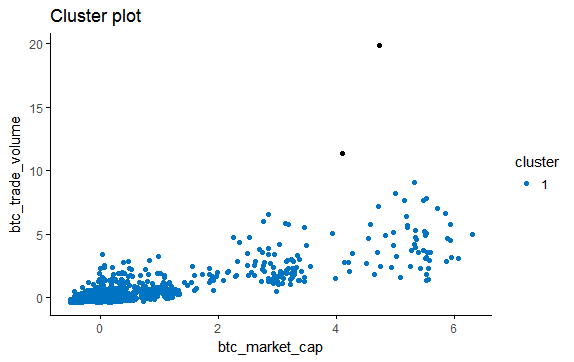
\includegraphics[width=10cm]{dbmarcapvolFig8.png}
    \caption{DBSCAN Clustering for Market Cap and Trade Volume }
    \label{fig:my_label}
\end{figure}


\section{Association Rules Mining}
Association rule learning is a rule-based machine learning method for discovering interesting relations between variables in large databases. It is intended to identify strong rules discovered in databases using some measures of interestingness It is often used by grocery stores, retailers, and anyone with a large transactional databases.Association rules use the R arules library. The arulesViz add additional features for graphing and plotting the rules. 

We have considered the Bitcoin Data Set which has 24 features or attributes in it. We have extracted 16 important features and build a subset of the data.First we have converted our dataset to transactions which is necessary step for rule creation. The rules can then be created using the Apriori function on the transaction dataset. After running the Apriori Function 860931 rules were created and the following statistics were obtained; Confidence of 0.8 and Minimum Support count of 292. The figure 15 illustrates it. \newline

\begin{figure}[h]
    \centering
    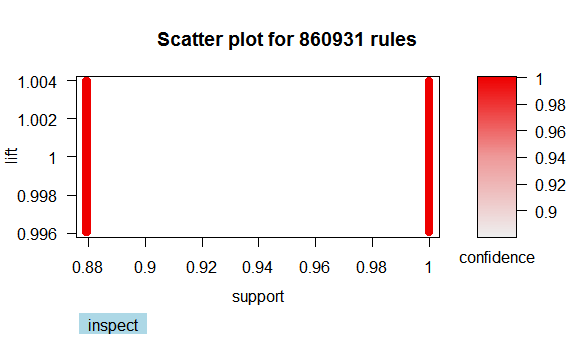
\includegraphics[width=10cm]{RuleMiningScatterPlotFig9.png}
    \caption{ Association Rule Mining Scatter Plot }
    \label{fig:my_label}
\end{figure}

 We can now create the subset of rules to visualise the set of rules. Every rule is composed by two different sets of items, also known as itemsets,  X and Y, where X is called antecedent or left-hand-side (LHS) and Y consequent or right-hand-side (RHS).From figure 17 we get these graphs we can see the two parts to an association rule: the antecedent (IF) and the consequent (THEN).  These patterns are found by determining frequent patterns in the data and these are identified by the support and confidence.  The support indicates how frequently the items appear in the dataset. The confidence indicates the number of times the IF/THEN statement on the data are true.These IF/THEN statements can be visualized by the following graph. \newline

\begin{figure}[h]
    \centering
    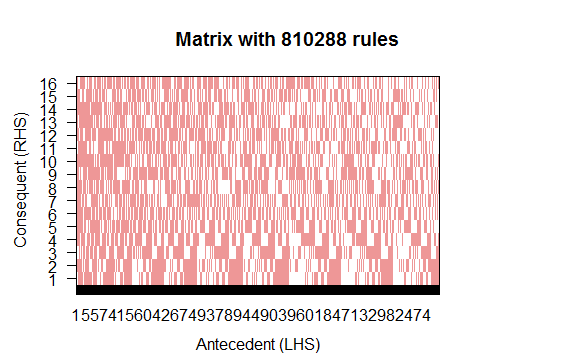
\includegraphics[width=6cm]{AntecedentConsequentFig11.png}
    \caption{Antecedent Consequent for the Subrules Created}
    \label{fig:my_label}
\end{figure}


 \begin{figure}[h]
    \centering
    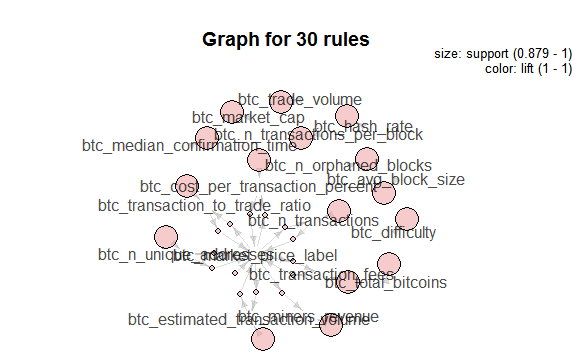
\includegraphics[width=10cm]{Graphfor30RulesFig12.png}
    \caption{Graph for 30 Rules}
    \label{fig:my_label}
\end{figure}

We can then subset the rules to the top 30 most important rules and then inspect the smaller set of rules individually to determine where there are meaningful associations. We plot the graph as in the above figure for top 30 rules and inspect them to find meaningful correlation between different attributes based on LHS and RHS. In practical applications, a rule needs a support of several hundred transactions before it can be considered statistically significant and datasets often contain thousands or millions of transactions.

\newpage

\section{Time Series Analysis}

\subsection{Introduction}

Time Series data is the collection of observations which are collected over a period of time, generally over fixed intervals. The data can be divided into univariate or multi-variable based on number of attributes. Time series data analysis is applied for the purpose of:

\begin{itemize}
	\item Understanding what happened in the past (Trend).
	\item Predicting/Forecasting the future.
\end{itemize}

\subsection{Stationary Series}
One of the basic requirement for time series modeling is to first check whether the data is stationary or non-stationary. The data is said to be stationary if it satisfies the following  property:

\begin{itemize}
	\item The mean of the series should not be a function of time but should be a constant.
	\item The variance of the series should not be a function of time.
	\item The co-variance of the ith term and (i + m)th term should not be a function of time.
\end{itemize}

So, for the time series modeling, if the data is not stationary, it has to be first converted into stationary data.
To verify whether data is stationary or not, we can use Dickey Fuller Test of Stationarity.
For the Dickey-Fuller Test, the p value has to be less than 0.05 or 5.
If it satisfies the above condition, it is considered as stationary series, else it is a non-stationary series.
To convert non-stationary into stationary, differencing should be applied before proceeding.


\subsection{Time Series Components}
There are four components of the Time Series:

\begin{itemize}
	\item Trend Component:
	Movement of data over a period of time like whether increasing, decreasing or remaining unchanged are defined as Trend.
	\item Seasonal Component:
	Fluctuations observed during specific seasons or chunks of time e.g. during 4th quarter of very year, stocks tends to show better.
	\item Cycle Component:
	Some type of data tends to repeat itself over a longer period of time, thereby exhibiting some cycles. It can be combination of trend and seasonal data.
	\item Irregular Component:
	Randomness or noise in the data.
\end{itemize}	

The time series modelling can be represented as additive or multiplicative model.
Additive Model:
\begin{equation}
Y(t) = T(t) + S(t) + C(t) + R(t)
\end{equation}
Multiplicative Model:
\begin{equation}
Y(t) = T(t) * S(t) * C(t) * R(t)
\end{equation}
where, T - Trend, S - Seasonal, C - Cycle, R - Random

\subsection{Identify p, d and q for ARIMA/Multivariate-ARIMA models}
	
	The two key concepts which helps in identifying the p and q values used in AR(p) and MA(q), are ACF and PACF
	
	\subsubsection{Autocorrelation Function(ACF)}
	It is a correlation function which rather than showing correlation between two different variables, shows the correlation between different values of same variable i.e X$_{i}$ and X$_{i+k}$.\linebreak
	ACF is used to identify the q value for \textbf{MA} component of ARIMA/Multivariate-ARIMA. To calculate the MA term of the model, the lag at which the ACF cuts is considered. It displays the sharp cut-off at the negative correlation.

	
\subsubsection{Partial Autocorrelation Function(PACF)}

It is also a correlation function, but it gives the partial correlation of time series with its own lagged values, controlling for the values of the time series at all shorter lags. It contrasts with the autocorrelation function, which does not control the other lags.\linebreak
PACF is used to identify the p value for the AR component of ARIMA/Multivariate-ARIMA.
The lag at which the PACF cuts off is the indicated number of AR terms. It displays a sharp cutoff at the positive autocorrelation.

\subsection{Finalizing values for p, d and q}

\begin{itemize}
	\item p - This is calculated by finding the lag k via PACF function
	\item d - This is the differencing order used while making the data stationary.
	\item q - This is calculated by finding the lag k via ACF function.
\end{itemize}

\subsection{Generating ARIMA model}

After identifying the values of p, d and q, we can create the ARIMA/Multivariate-ARIMA models.
The ARIMA model can then be used to forecast or predict the future values.\linebreak

ARIMA model can be validated by examining ACF and PACF for residual models.
After fitting the correct model, it can then be used to do forecast and prediction.\linebreak
We can also verify the forecast and prediction, by reserving a portion of our dataset and applying the prediction on top of it, thereby comparing the forecasted and actual
observed values.

\section{Application of ARIMA/Multivariate-ARIMA models}

\subsection{ARIMA Model}
Dataset used: bitcoin\_price.csv  \linebreak
Attribute used for modelling - Close Price  \linebreak
ARIMA model - univariate analysis as trading prices are often analyzed based on how they had been behaving over the period of time. \linebreak
Data has been cleaned before applying ARIMA/Multivariate-ARIMA model. \linebreak

\subsubsection{Exploring Raw Data}

Plot for visualizing the raw data as obtained is shown in Figure 18.
\begin{figure}[ht]
	\centering
	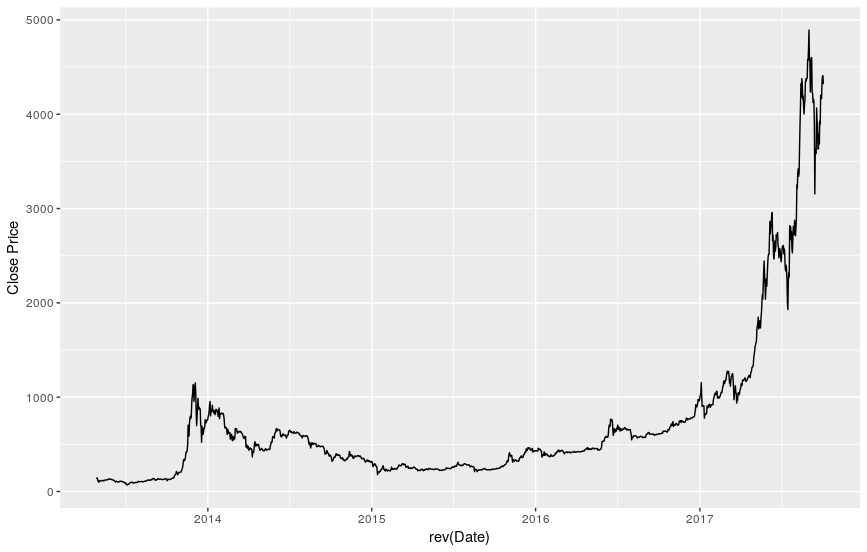
\includegraphics[scale=0.30]{RawClosePricePlot.png}
	\caption{Original Raw Close Price Data}
	\label{fig:Original Raw Close Price Data}
\end{figure}

With the K-Means clustering it was identified, that there existed some outliers.
So, with tsclean function of R, data has been cleaned for outliers to avoid any skewing.\linebreak Figure 19 shows clean data.

\begin{figure}[ht]
	\centering
	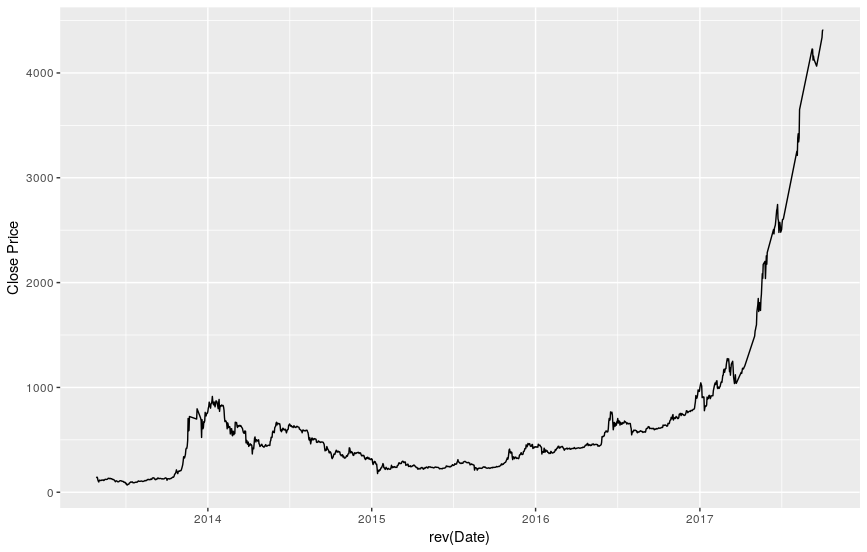
\includegraphics[width = 6cm]{CleanedClosePricePlot.png}
	\caption{Cleaned Close Price Data}
	\label{fig:Cleaned Close Price Data}
\end{figure}


As part of exploration, we also calculated the moving average data. However, this moving average was to smoothen the data rather than actual modelling.
Further analysis is done on dataset with this moving average value.\linebreak Figure 20. shows the smoothened data.

\begin{figure}[ht]
	\centering
	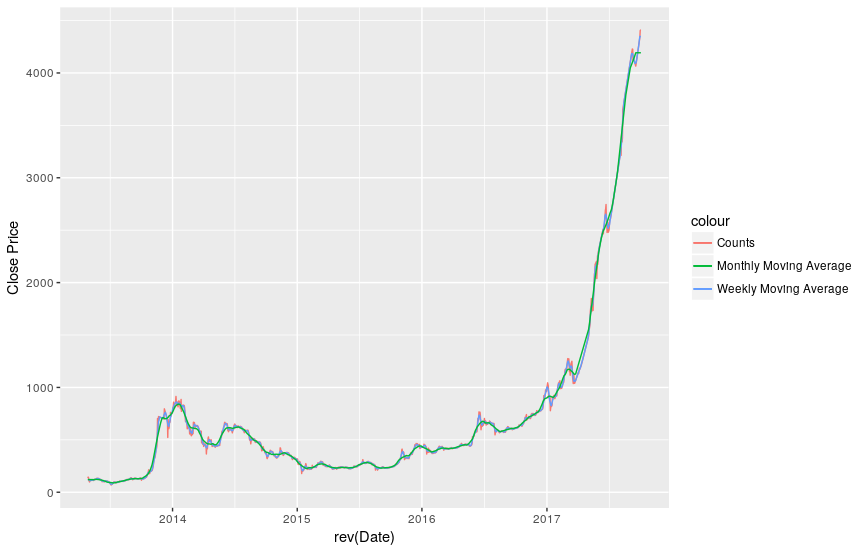
\includegraphics[width = 6cm]{MovingWeeklyAverage.png}
	\caption{Moving Average Data}
	\label{fig:Moving Average Data}
\end{figure}
\newpage
\subsubsection{Trend Components}
Figure 21 shows the trend, seasonal and residual components for the dataset.

\begin{figure}[ht]
	\centering
	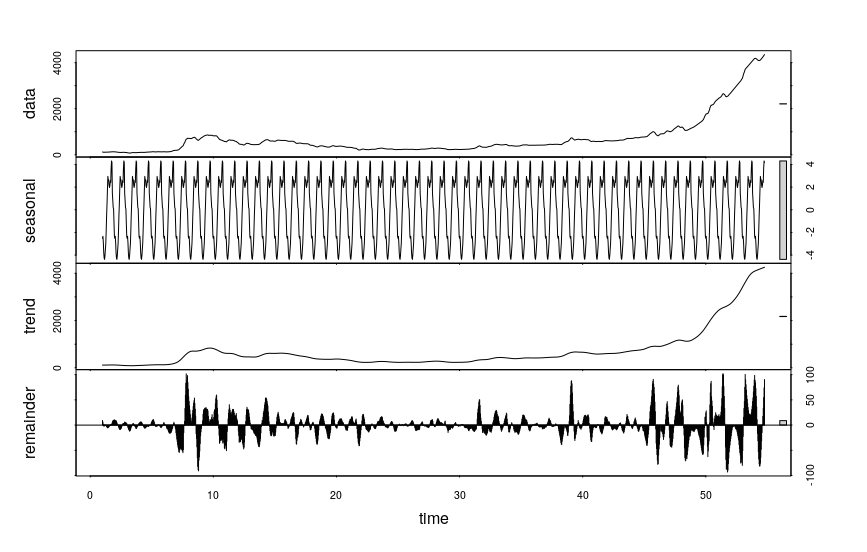
\includegraphics[width = 6cm]{TimeSeriesComponents.png}
	\caption{Time Series Components}
	\label{fig:Time Series Components}
\end{figure}

Since there did exist some seasonal component, we subtracted it as shown in Figure 22.


\begin{figure}[ht]
	\centering
	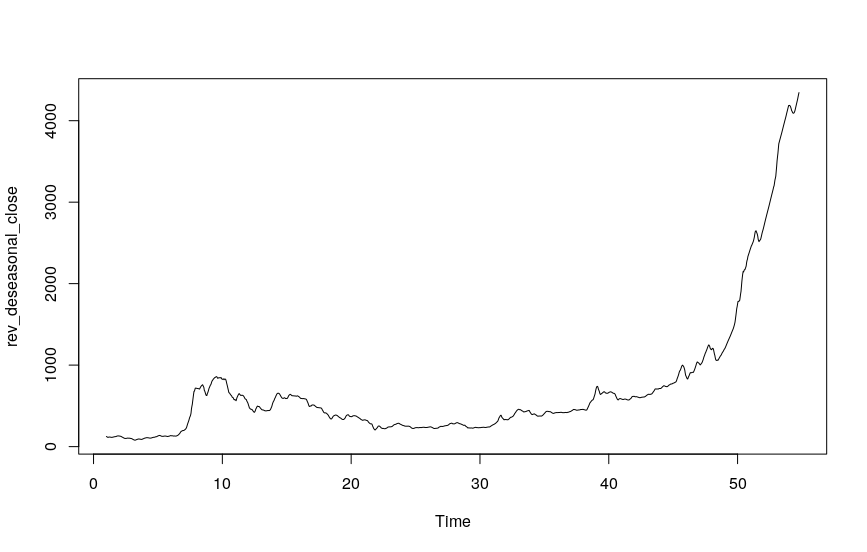
\includegraphics[width = 6cm]{SubtractingSeasonal.png}
	\caption{Subtracting Seasonal Components}
	\label{fig:Subtracting Seasonal Components}
\end{figure}

Further analysis is done on data after subtracting seasonal components.
\newpage
\subsubsection{Stationary Series}

Next step identifies if the data is stationary or not, by applying Dickey Fuller Test and verifying with Plot.
\\ \textbf{Differencing 0}
Without any differencing, the result of Dickery Fuller Test, showed following value

p-value = 0.99, Alternative Hypothesis: stationary
 \\ Since p-value > 0.05, it implies that there is a need of differencing. It can also be seen from Figure (Cleaned Close Price Data)
This is applied without differencing so it is same as Figure 3.

\\ \textbf{Differencing 1}
Differencing value as 1, the result of Dickery Fuller Test, showed following value

p-value = 0.01, Alternative Hypothesis: stationary 
Since p-value < 0.05, it implies that data is now stationary, also seen from Figure 23 for differenced Close Price Data.

\begin{figure}[ht]
	\centering
	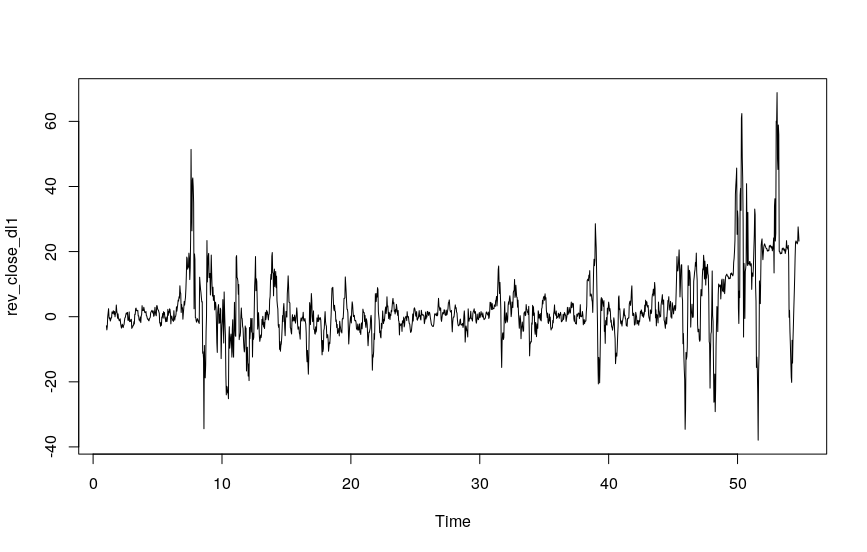
\includegraphics[width=6cm]{CloseWithDifferencing1.png}
	\caption{Close Price after 1 order differencing}
	\label{fig:Close Price after 1 order differencing}
\end{figure}

\\ \textbf{Differencing 2}
Differencing value as 2, the result of Dickery Fuller Test, showed following value

\\ p-value = 0.01, Alternative Hypothesis: stationary
Since p-value < 0.05, it implies that data is now stationary, also seen from Figure 24 for differenced Close Price Data.

\begin{figure}[ht]
	\centering
	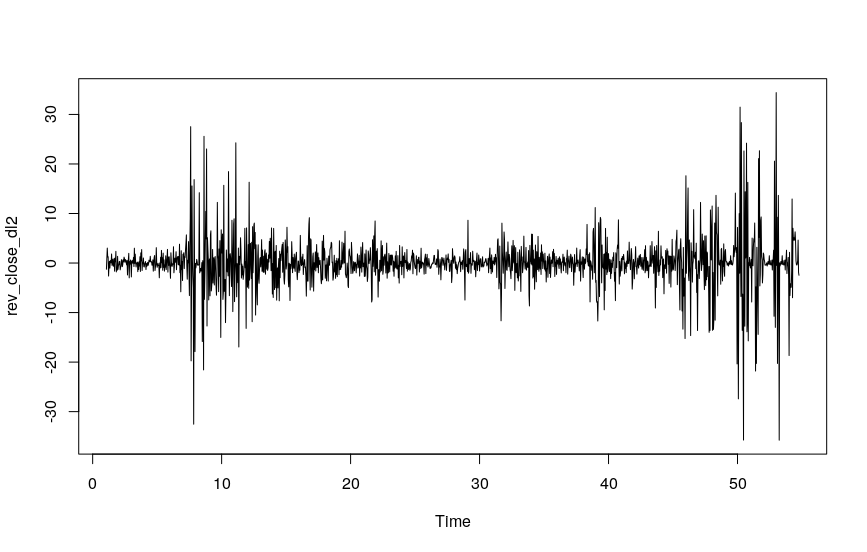
\includegraphics[width=6cm]{CloseWithDifferencing2.png}
	\caption{Close Price after 2 order differencing}
	\label{fig:Close Price after 2 order differencing}
\end{figure}


Since both with d = 1 and d = 2, we get p < 0.01, we can choose any of these for further analysis. However, if we see the plots we see that the graph with d = 2 is more around 0 value rather than d = 1. And so we 
decide to take d = 2 for further analysis.

\newpage
\subsubsection{Identify p, d and q for ARIMA models}

\\ \textbf{ACF and PACF for Differencing 0}

Figure 25 and 26 shows ACF and PACF plots for data without any differencing.

\begin{figure}[ht]
	\centering
	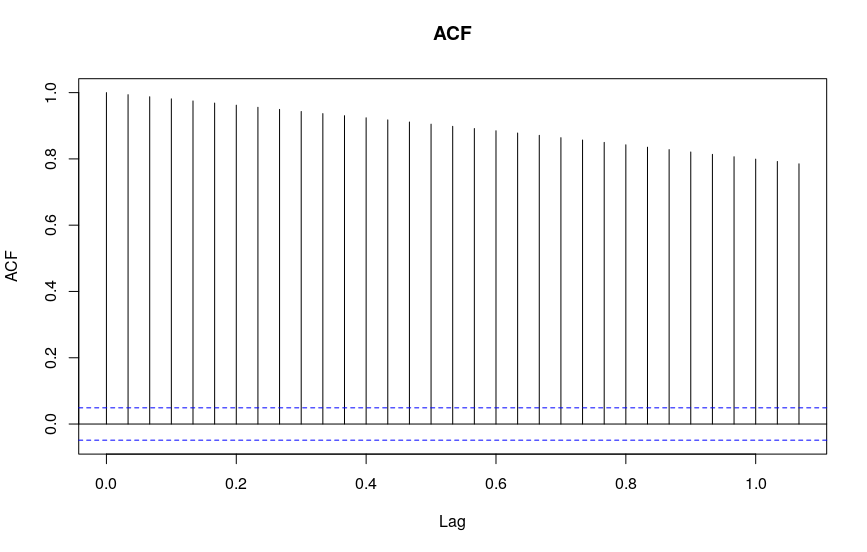
\includegraphics[width=6cm]{ACFWith0Differencing.png}
	\caption{ACF with 0 order differencing}
	\label{fig: ACF with 0 order differencing}
\end{figure}
\newpage
\begin{figure}[ht]
	\centering
	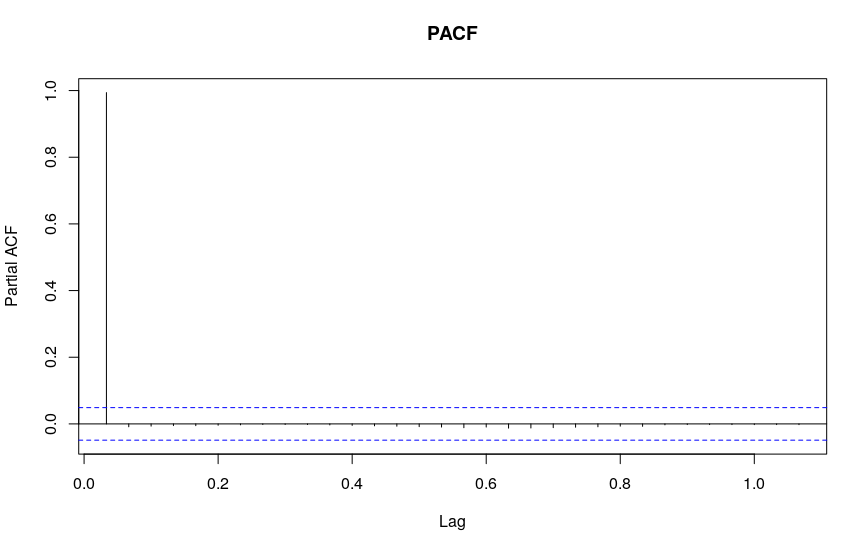
\includegraphics[width=6cm]{PACFWith0Differencing.png}
	\caption{PACF with 0 order differencing}
	\label{fig: PACF with 0 order differencing}
\end{figure}

\\ \textbf{ACF and PACF for Differencing 1}

Figure 27 and 28 shows ACF and PACF plots for data with differencing order 1.

\begin{figure}[ht]
	\centering
	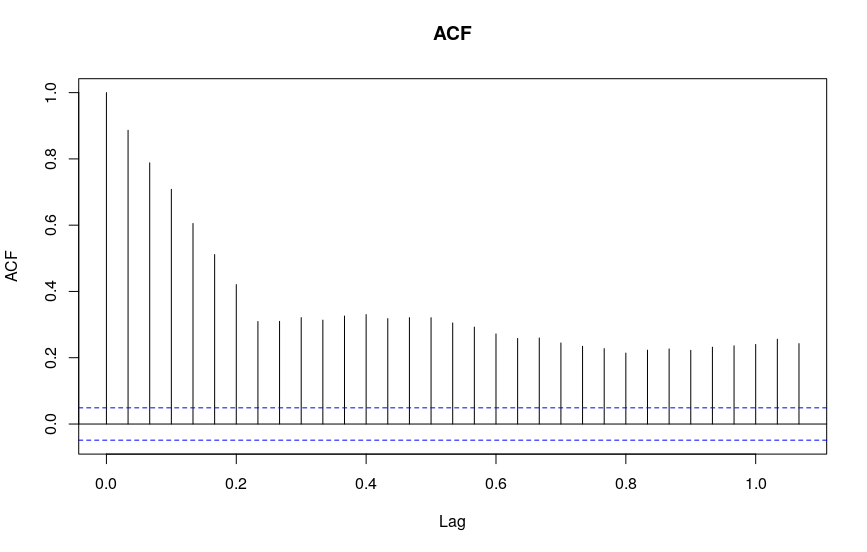
\includegraphics[width=6cm]{ACFWith1Differencing.png}
	\caption{ACF with 1 order differencing}
	\label{fig: ACF with 1 order differencing}
\end{figure}
\newpage
\begin{figure}[ht]
	\centering
	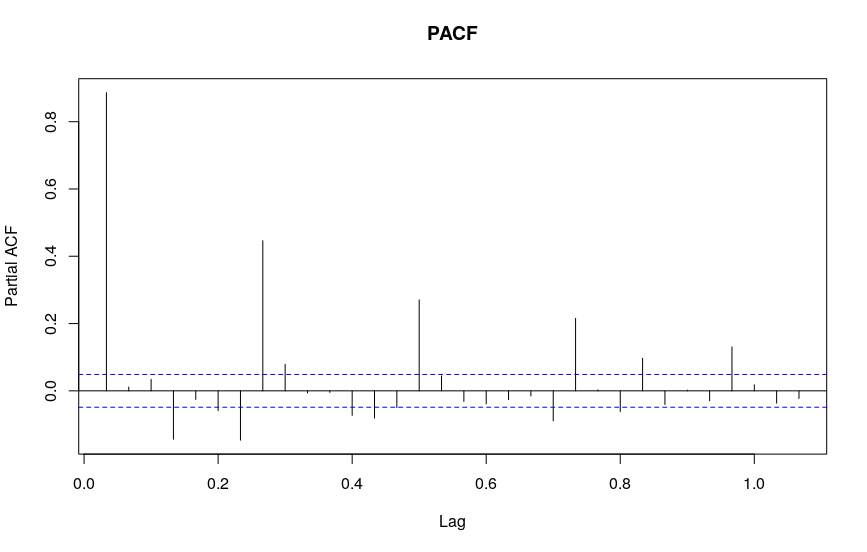
\includegraphics[width=6cm]{PACFWith1Differencing.png}
	\caption{PACF with 1 order differencing}
	\label{fig: PACF with 1 order differencing}
\end{figure}

\\ \textbf{ACF and PACF for Differencing 2}

Figure 29 and Figure 30 shows ACF and PACF for data with differencing order 2.

\begin{figure}[ht]
	\centering
	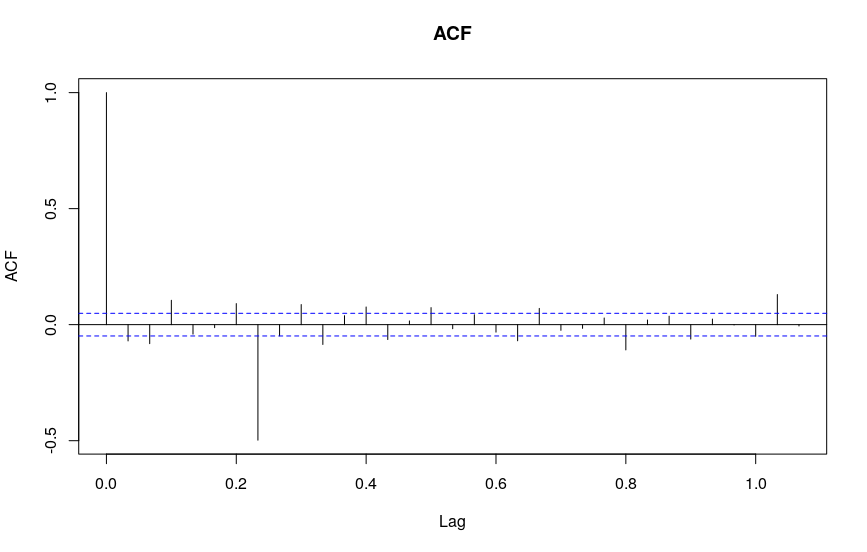
\includegraphics[width=6cm]{ACFWith2Differencing.png}
	\caption{ACF with 2 order differencing}
	\label{fig: ACF with 2 order differencing}
\end{figure}

\begin{figure}[ht]
	\centering
	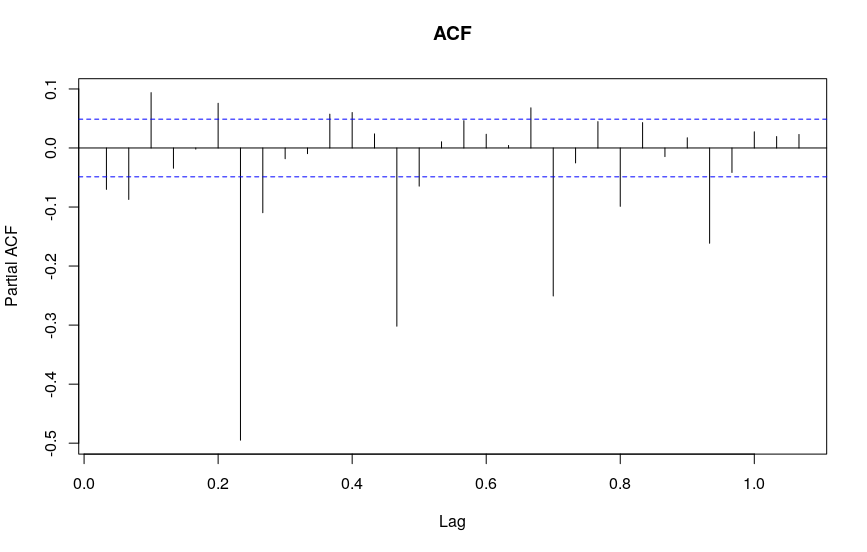
\includegraphics[width=6cm]{PACFWith2Differencing.png}
	\caption{PACF with 2 order differencing}
	\label{fig: PACF with 2 order differencing}
\end{figure}

We can see ACF and PACF plots for differencing order 1, 2, and 3 as above. And we see that ACF plot shows the lags in the graph with d = 2.
So, this again matches with our previous conclusion when we considered the stationary data for d = 2.
With this we take p = 3 from ACF and q = 7 from PACF as that is where we see real positive and negative correlation sharp cut-off respectively.

\subsubsubsection{Generating ARIMA model}
With p = 3, d = 2, and q = 7, we have following ARIMA model generated as shown in Figure 31.

\begin{figure}[ht]
	\centering
	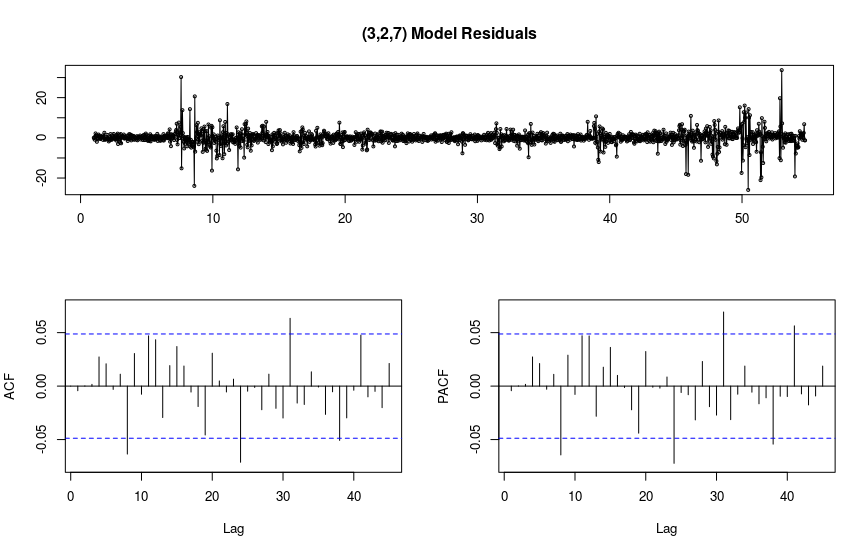
\includegraphics[width=6cm]{ARIMAWith327.png}
	\caption{ARIMA with 3,2,7}
	\label{fig: ARIMA with (3,2,7)}
\end{figure}

\newpage
\subsubsection{Forecasting}

After generating the above model, we did the forecasting for next 25 elements.

Figure 32 shows the 

\begin{figure}[ht]
	\centering
	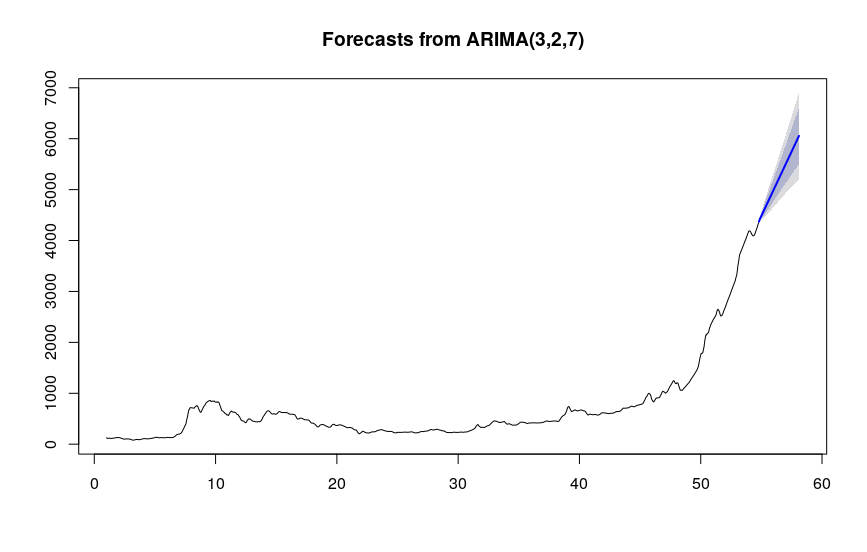
\includegraphics[scale=0.25]{ForecastWith327.png}
	\caption{ARIMA with 3,2,7}
	\label{fig: Forecast with ARIMA(3,2,7)}
\end{figure}

To confirm the model, we did the forecast for a part of existing data and see how it compares with original data as shown in Figure 33.

\begin{figure}[ht]
	\centering
	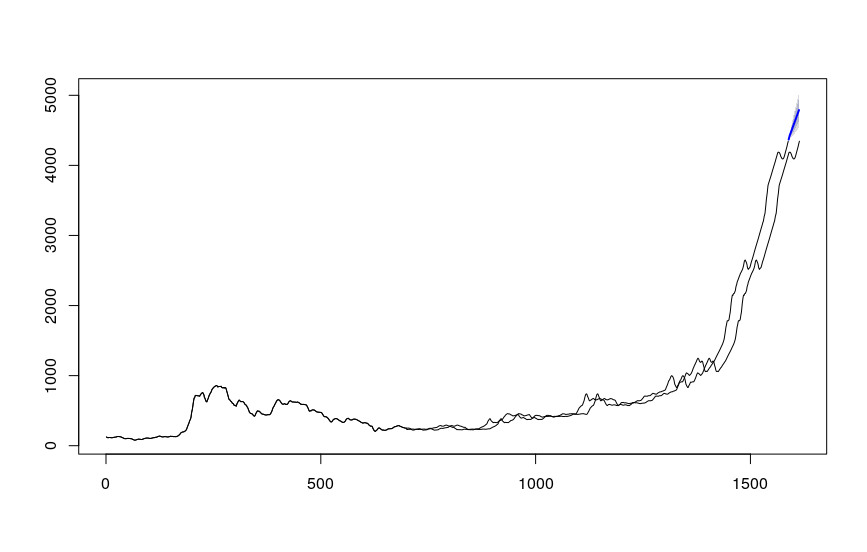
\includegraphics[scale=0.25]{ForecastedImageH25.png}
	\caption{Forecast and comparision with original data}
	\label{fig: Forecast and Comparision with original data}
\end{figure}

Last we tried future trend prediction which matches with our original trend as shown in Figure 34.

\begin{figure}[ht]
	\centering
	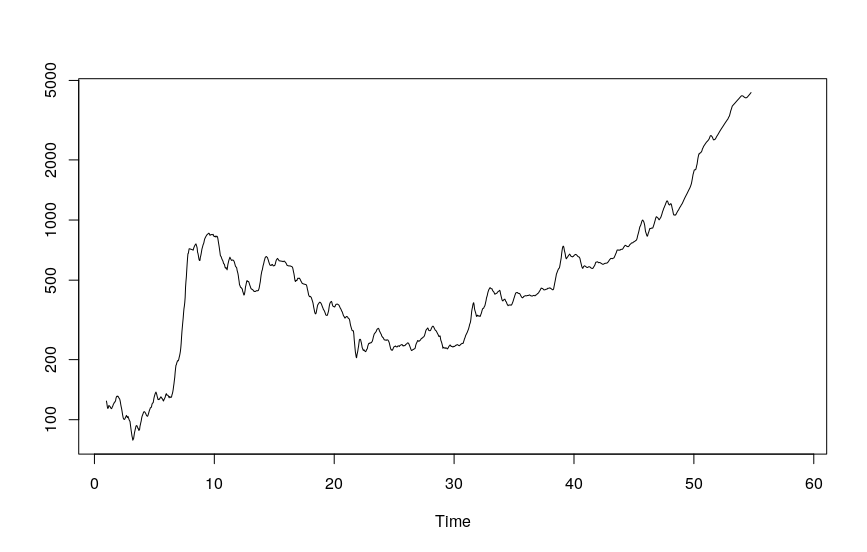
\includegraphics[scale=0.25]{FutureTrendPrediction.png}
	\caption{Future Trend Prediction}
	\label{fig: Future Trend Prediction}
\end{figure}

\newpage

\subsection{Multivariate-ARIMA Model}
Multivariate-ARIMA model is applied on time-series data containing multiple attributes as opposed to univarate time series in ARIMA model. The marima model has been applied to \textbf{ethereum price} dataset. As explained above, non stationary dataset is made stationary to perform time series analysis. Different differencing techniques were applied and plotted. Difference(of order 1) of log of data and difference(of order 1) of square root of data seemed to show the constant variance in data. Hence the data was reduced into one of the former and was converted into a time-series object. For defining the marima model, ACF/PACF plots were used to check the lag values for AR and MA components of the model. The Date attribute was removed from the defined model for further time series analysis and one of the attributes (i.e. Close, Open, High, Low and Market Capitalization) were chosen as regression variables. A penalty is defined in the interval [0, 2] for stepwise model reduction i.e. defining the level of significance to consider AR and MA parameters in estimating the accurate model. As stated above, some data points were reserved for forecasting through the estimated model. Two models were created i.e. one with the normalized and non-stationary dataset without the differencing and other on the differenced/stabilized data. 

The plot below shows the trend of bitcoin dataset features (such as Open, Close, High, Low, etc) with time. Non Linearity of attributes can be seen from the first and second plots. The non stationarity of the attributes can still be seen after doing the first order differencing. However, after applying difference of either log or square root transformating, the data becomes stationary, as visible in the third plot.
\begin{figure}[ht]
	\centering
	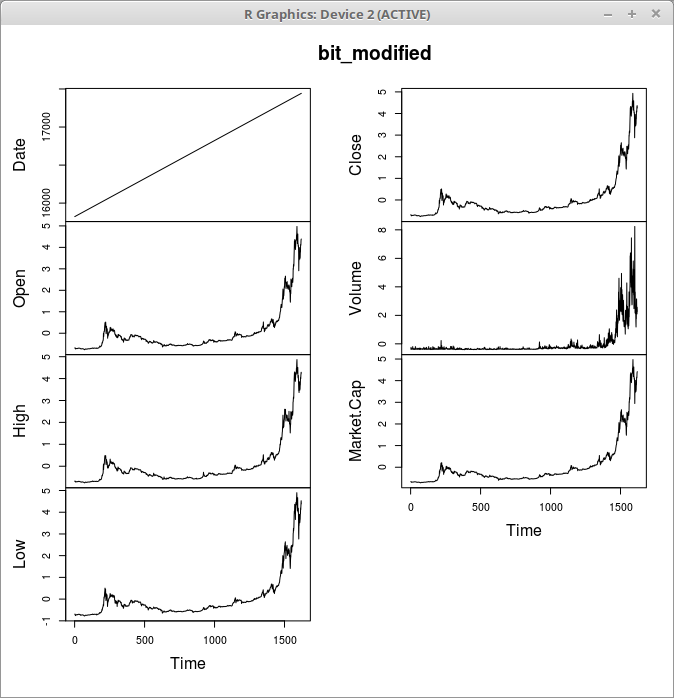
\includegraphics[width = 6 cm]{btc_attributes.png}
	\caption{Original trends of bitcoin attributes}
	\label{fig: btc_attri}
\end{figure}

\begin{figure}[ht]
	\centering
	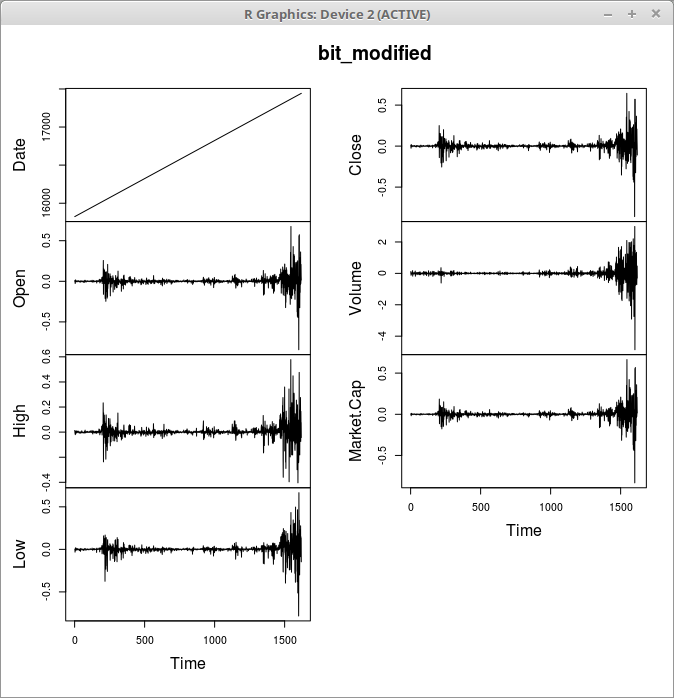
\includegraphics[width = 6 cm]{btc_non_stationary_attributes.png}
	\caption{Trends of bitcoin attributes after first order differencing}
	\label{fig: btc_non_stat_attr}
\end{figure}
\newpage

\begin{figure}[ht]
	\centering
	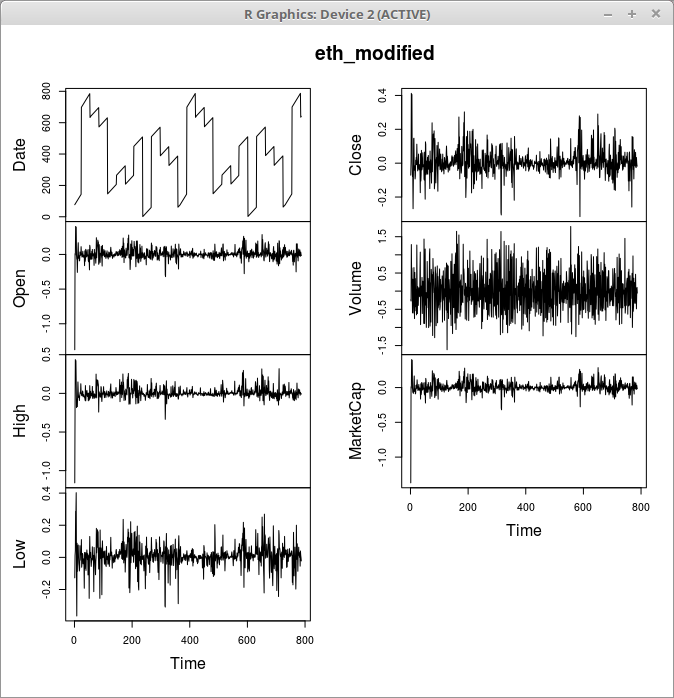
\includegraphics[width = 6 cm]{btc_differenced attributes.png}
	\caption{Trends of stationary bitcoin attributes}
	\label{fig: btc_diff_attri}
\end{figure}


The ACF plot of residuals is caclulated bolow to get approximate values of p and q values for respective AR and MA components of MARIMA model for accurate estimation.
\begin{figure}[ht]
	\centering
	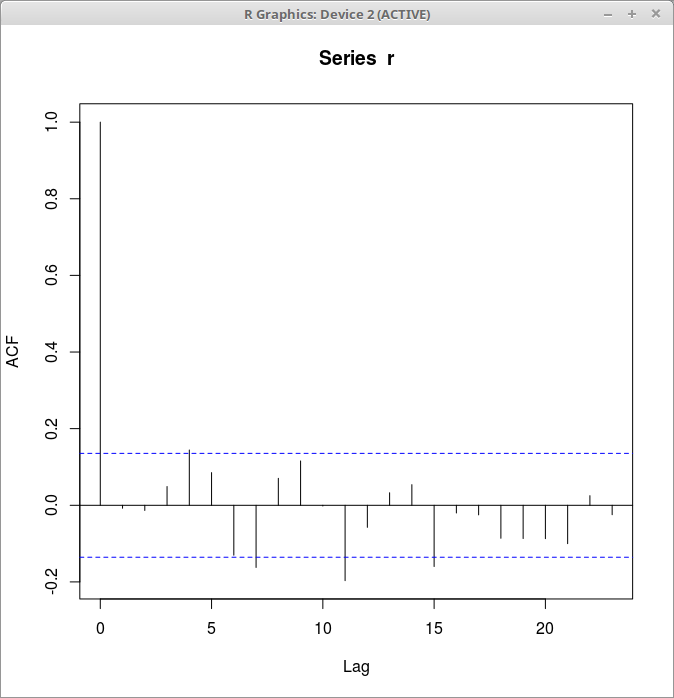
\includegraphics[width = 6 cm]{residual_acf.png}
	\caption{ACF Plot for residual on bitcoin data}
	\label{fig: resi_acf}
\end{figure}

\newpage
The plots below shows the forecasting done for Close and Market Capitalization attributes, on the non stationary as well as stationary data from the estimated MARIMA model. The black line shows the ground truth with the green line showing the results of forecasting.
\begin{figure}[ht]
	\centering
	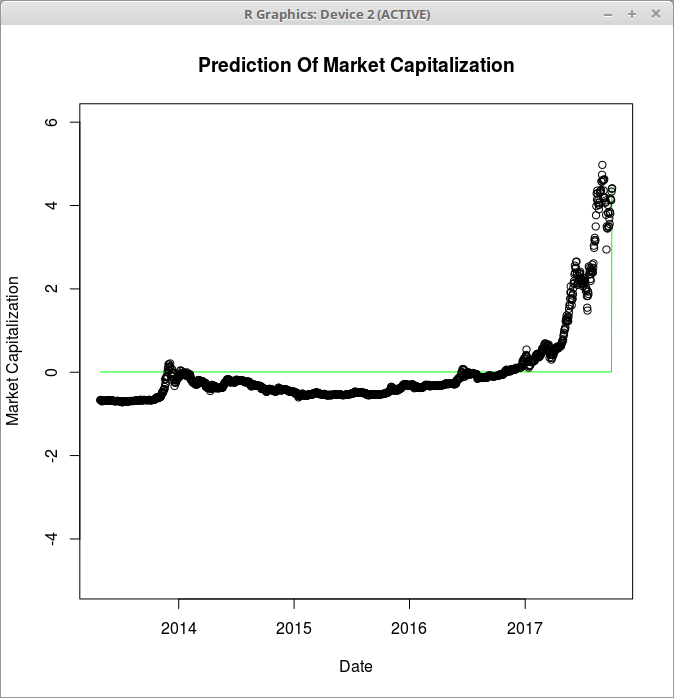
\includegraphics[width = 6 cm]{market_cap_prediction.png}
	\caption{Forecasting of Market Capitalization}
	\label{fig: btc_non_stat_pred}
\end{figure}

\begin{figure}[ht]
	\centering
	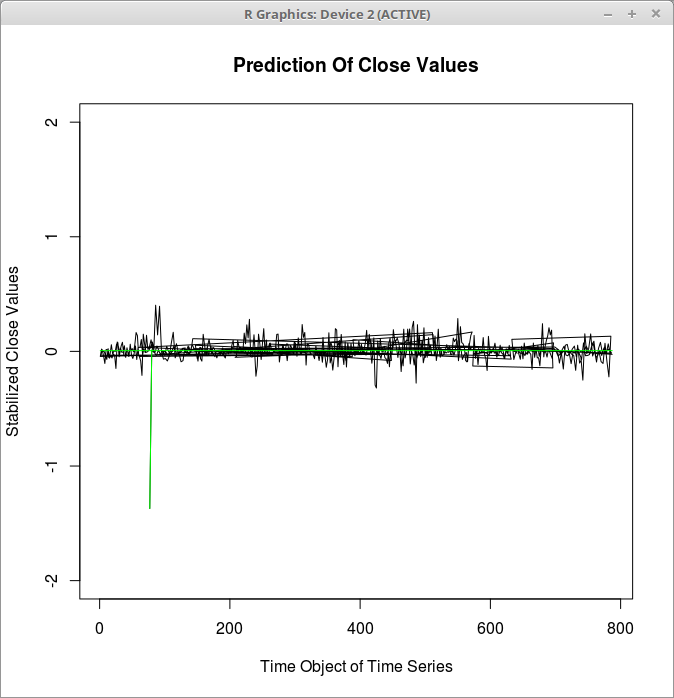
\includegraphics[width = 6 cm]{stationary_btc_prediction.png}
	\caption{Forecasting of Close Attribute}
	\label{fig: btc_stat_pred}
\end{figure}

\newpage

\begin{thebibliography}{widestlabel}
	
	\bibitem{1}
	STOCK MARKET TRENDS USING CLUSTER ANALYSIS AND ARIMA MODEL by Joyti Badge, Published in stock Market Trends
	Asian-African Journal using of Economics Cluster Analysis
	and Econometrics, and ARIMA Model Vol. 13, No. 2, 2013: 303-308
	
	\bibitem{2}
	ANALYSIS OF NIFTY FIFTY STOCKS BASED ON K-MEANS CLUSTERING TECHNIQUE FOR STOCK MARKET PREDICTION Dr. T.Chitra kalarani* and S.Indrakala**
	
	\bibitem{3}
	Book named "Data Mining Concepts and Techniques", Jiawei Han, Micheline Kamber, Jian Pei
	
	\bibitem{4}
	https://www.datascience.com/blog/introduction-to-forecasting-with-arima-in-r-learn-data-science-tutorials
	
	\bibitem{5}
	https://www.analyticsvidhya.com/blog/2015/12/complete-tutorial-time-series-modeling/
	
	\bibitem{6}
	https://www.slideshare.net/21\_venkat/arima-26196965
	
	\bibitem{7}
	https://people.duke.edu/~rnau/411arim3.htm
	
	\bibitem{8}
	https://www.openml.org/a/estimation-procedures/1
	
	\bibitem{9}
	https://en.wikipedia.org/wiki/Dimensionality\_reduction
	
\end{thebibliography}

\end{document}